\documentclass[a4paper]{report}

\usepackage{natbib}
\usepackage{graphicx}
\usepackage[pdfborder={0 0 0}]{hyperref}
\usepackage{pdfpages}

\usepackage[T1]{fontenc}
\usepackage[sc]{mathpazo}

\lefthyphenmin 5
\righthyphenmin 5


\begin{document}

\begin{titlepage}
% {{{
\begin{center}

\textsc{\Large Honours Project Report \\
\ \\
\ \\
\ \\
\ \\
\ \\
}

{\huge \bfseries
Water Compression Visualisation
\\}

\vfill

\large Min-Young Wu
\\
\small{mwu@cs.uct.ac.za}

\ \\
\ \\

\begin{tabular}{cc}
  \multicolumn{2}{c}{\large Supervised By:} \\
  \\
  \large Patrick Marais & \large James Gain
  \\
  \small patrick@cs.uct.ac.za & \small jgain@cs.uct.ac.za
\end{tabular}

\vfill

\begin{tabular}{|l|l|c|}
  \hline
  & \textbf{Category} & \textbf{Chosen} \\
  \hline
  1 & Software Engineering/System Analysis & 5 \\
  \hline
  2 & Theoretical Analysis & 0 \\
  \hline
  3 & Experiment Design and Execution & 15 \\
  \hline
  4 & System Development and Implementation & 5 \\
  \hline
  5 & Results, Findings and Conclusion & 15 \\
  \hline
  6 & Aim Formulation and Background Work & 10 \\
  \hline
  7 & Quality of Report Writing and Presentation & 10 \\
  \hline
  8 & Adherence to Project Proposal and Quality of Deliverables & 10 \\
  \hline
  9 & Overall General Project Evaluation & 10 \\
  \hline
  \multicolumn{2}{|l|}{\textbf{Total marks}} & 80 \\
  \hline
\end{tabular}

\vfill

\textsc{\Large Department of Computer Science \\
\ \\
University of Cape Town \\
\ \\}

{\large 2009}

\end{center}
\end{titlepage}
% }}}

\setlength{\parskip}{3mm plus2mm minus1mm}
\thispagestyle{empty}

\section*{Abstract}
% {{{

Molecular simulations generates large amounts of data, over many days. Being
able to compress this data will be advantageous; both for storage, as well as
data transmission. Performing compression by taking advantage of certain
characteristics of the data is expected to yield promising results. The water
compression project aims to achieve high compression ratios by exploiting the
presence of large amounts of water in the simulation.

The visualisation aspect of the water compression project is there to support
the main compression goal of the system. To facilitate compression, the
molecular data is quantised, floating point values gets mapped to integer
values. Thus, the visualisation aspect has been split up into two main parts:
visualisation of the molecular data, and an experiment to measure the
perceptual impact of quantisation.

A number of different visualisation techniques has been developed in order to
visualise the molecular data, two of which was used in the quantisation
experiment. The quantisation experiment results indicates that 8 and 10 bit
quantisation yields results that are perceived to be similar to the original
data. Further quantisation, 6 and 4 bit quantisation, yields results that are
rated different and very different.

\ \\
\ \\
\ \\

\textbf{Categories:} \\
H.5.2 [User Interfaces] Graphical user interfaces (GUI)

\textbf{Keywords:} \\
Visualisation

% }}}



\setcounter{page}{1}
\pagenumbering{roman}
\setlength{\parskip}{0mm plus5mm minus0mm}
\tableofcontents
\listoffigures
\listoftables

\newpage
\setcounter{page}{1}
\pagenumbering{arabic}

\setlength{\parskip}{3mm plus2mm minus1mm}
\graphicspath{{./introduction/}}

\chapter{Introduction}
% {{{
\label{cha:introduction}

Molecular simulations typically generate massive amounts of data. A large
simulation can comprise hundreds of thousands of atoms, with thousands of
frames, yielding many gigabytes of data. Due to the computational costs and
time required to perform these simulations, they are often run on clusters,
which means that the generated data needs to be transferred from the cluster to
a researchers' workstation. Compressing the molecular data is thus advantageous
as it will make transferring the data faster, as well as decreasing the storage
costs.

As water is the solvent in which many molecular simulations occur in, a large
proportion of the volume in these simulations is water. Water has certain
structural properties that can be exploited to achieve good compression ratios.
The water compression project thus targets molecular simulations with large
amounts of water, aiming to achieve high compression ratios by exploiting these
properties.

\section{Overview}
% {{{
\label{sec:introduction_overview}

Molecular simulations are composed of a sequence of frames of data, a single
frame is a snapshot of the positions of all the atoms. Compressing molecular
simulations can thus be broken up into: compressing single frames (intraframe
compression), and compressing data across frames (interframe compression).

Our water compression project has been split into three main parts:

\begin{itemize}
  \item Intraframe compression
  \item Interframe compression
  \item Visualisation
\end{itemize}

The water molecules in a body of water do not group uniformly in all
directions; instead the water molecules form clusters. The presence of these
water clusters is used by the intraframe compressor to perform prediction.

The interframe compression is more general, it compresses all the atom
information, water and non-water molecules. Using previous frames of data, the
position of atoms in the next frame is predicted, and the error is encoded.

The visualisation aspect of the project supports the main goal of the project:
compressing molecular simulations. To do so, the molecular simulation data will
need to be visualised, and a quantisation experiment carried out. Section
\ref{sec:introduction_quantisation} introduces and explains the need for the
quantisation experiment. Section \ref{sec:introduction_visualisation}
introduces the visualisation infrastructure developed for the quantisation
experiment.

This report will focus on the visualisation aspect of the water compression
project. The intraframe and interframe components of the system are handled in
their respective reports.

% }}}

\section{Quantisation Experiment}
% {{{
\label{sec:introduction_quantisation}

Quantisation maps floating point values onto integer values, ranges of floating
point values are mapped to different integer values. Quantising point data
will have the effect of snapping the points to a grid. Figure
\ref{fig:introduction_quantisation} illustrates the effects of quantisation;
unquantised points are shown in the left image, the quantised points are in the
right image.

\begin{figure}
  \begin{center}
    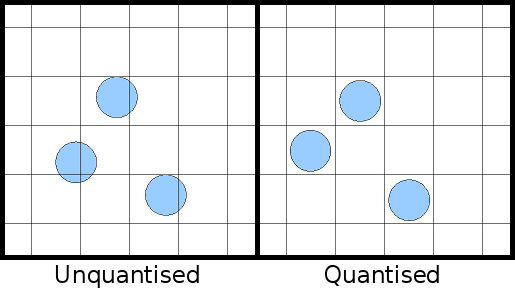
\includegraphics[width=100mm]{quantisation}
  \end{center}
  \caption{Diagram showing unquantised points (left) and quantised points
  (right).}
  \label{fig:introduction_quantisation}
\end{figure}

Quantisation is used to facilitate compressing the molecular data, integer
values can be more effectively compressed than floating point values.
Quantisation using fewer bits will increase the compression ratio as there will
be fewer values to encode, but fewer values means that more deviation from the
original input data, more data is discarded. Quantisation is the only lossy
step in the compression process, the following steps in the compression process
are lossless, no data is discarded.

With quantisation, a balance needs to be established between data fidelity and
compression ratio. Determining this balance is the aim of the quantisation
experiment: what is an acceptable level of quantisation? The acceptable level
of quantisation is where the differences between the original and quantised
data are not significantly noticeable.

% }}}

\section{Visualisation}
% {{{
\label{sec:introduction_visualisation}

The other aspect to the visualisation component of the system is to provide
visualisations of the molecular data. The visualisations used in the
quantisation experiment supports the compression components of the system, and
can be used for simple molecular data visualisation.

Due to the specific uses that are needed by the project, an existing
visualisation package is insufficient. Specific visualisations such as showing
the water clusters used by the intraframe compressor or quantisation error are
not present. A separate visualisation component is thus developed to provide
the infrastructure needed for the quantisation experiment, as well as provide
the compression specific visualisations.

% }}}

\section{Outline}
% {{{
\label{sec:introduction_outline}

The remainder of this report is structured as follows:

Chapter \ref{cha:background} provides background on relevant visualisation
techniques that influenced the development of our visualisation.

Chapter \ref{cha:design} identifies and details a number of visualisation
solutions. The chapter explains why these approaches are chosen and the design
behind them. A few of the visualisation approaches are aimed purely at
supporting the compressors.

Chapter \ref{cha:implementation} provides implementation details on each of the
visualisation components.

The quantisation experiment is detailed in Chapter \ref{cha:experiment}.

The experiment results and analysis are in Chapter \ref{cha:results}.

Finally, Chapter \ref{cha:conclusion} concludes and summarises this report.

% }}}

% }}}


\graphicspath{{./background/}}

\chapter{Background}
% {{{
\label{cha:background}

% {{{

Information visualisation techniques are very domain specific; one type of
visualisation may work well for a particular scenario, but work quite poorly
when applied to another domain. The problem domain of this project is the
effective visualisation of point cloud data, more specifically, water molecules
from molecular simulations.

As water is the solvent in molecular simulations, it occupies much of the
volume. This poses the challenge on how to effectively visualise large amounts
of point data. Some of the important issues that need to be investigated are
the presentation of appropriate levels of detail and clutter control.

Section \ref{sec:background_molecular} identifies and briefly introduces
several molecular visualisation techniques, while Section
\ref{sec:background_general} focuses on more general visualisation techniques.
Section \ref{sec:background_summary} provides a short summary of the different
visualisation techniques.

% }}}

\section{Molecular visualisation}
% {{{
\label{sec:background_molecular}

% {{{

The most significant problem for visualising molecular data is the amount of
data available and how to represent it so as not to clutter up the display.
Some molecular visualisation techniques focus on simplifying the models by
analysing the data to identify structures, while others exclude certain data
from the visualisation. Either way, a simplified image is presented so as to
make the molecular data easier and quicker to understand.

Some of the visualisation techniques (ribbon, paper chain and twister) are
designed for very specific molecular data, and are thus not easily extensible
to point cloud data. They can, however, be used as an example to determine what
kind of analysis can be done on data to simplify and help identify structures.

It is worth mentioning the Visual Molecular Dynamics (VMD) \citep{humphrey96}
program, it is a commonly used visualisation package aimed at displaying,
animating and analysing large biomolecular systems \citep{VMD}. However, as VMD
is aimed at general biomolecular systems, support for specific visualisation
and filtering is limited. VMD does support and use some of the visualisation
techniques that are mentioned in this chapter.

% }}}

\paragraph{Ball-and-stick}
% {{{

The ball-and-stick model is the classical approach to representing molecular
structure. Colour coded spheres are used to represent the atoms, while
cylinders are used to represent the bonds between them. There are various
proposals for the colour scheme used in ball-and-stick representations
(\citep{rasmolcolour}, \citep{jmolcolour}, \citep{drumscolour}), but there is
no definite agreed upon standard. This model is used to emphasise the molecular
connectivity of the atoms. It is the one of the simpler approaches in molecular
visualisation and is most often used when much detail is required: typically
for looking at bond information, molecule orientation and reaction sites.

The problem with this model is that it does not handle large numbers of atoms
and bonds very well. Since all the atoms and bonds are visible, the view
quickly becomes crowded and overall structure is obscured. Occlusion of other
atoms often occurs and may hide important information. The ball-and-stick
representation is typically not used for large structures as it often produces
cluttered views, making it very difficult to understand and analyse the data.

% }}}

\paragraph{CPK}
% {{{

The CPK (Corey-Pauling-Koltun) \citep{corey53} representation simplifies the
ball-and-stick model by removing the cylinders used to represent bonds. The
spheres used for the atoms are enlarged to encompass the bonds. The atoms now
overlap with one another, covering up where the bonds would be.

Removing the bonds from the model simplifies the view and allows for the
overall shape and contour to be easily seen. Although this model has simplified
the ball-and-stick model, it does not highlight any structures, it has only
removed the bond information. In contrast, the later molecular visualisation
techniques in this section do highlight certain molecular structures.

The CPK representation is not well suited to the visualisation of large numbers
of molecules. As each of the atoms has been enlarged, each molecule occupies
more space than the ball-and-stick model; with the molecules being opaque, this
causes large areas to be occluded, which may hide important information and
make it hard to analyse an entire system.

Figure \ref{fig:background_ball_cpk} shows the ball-and-stick and CPK
representation of the same molecule. The ball-and-stick representation is on
the left, while the CPK representation is on the right.

\begin{figure}
  \begin{center}
    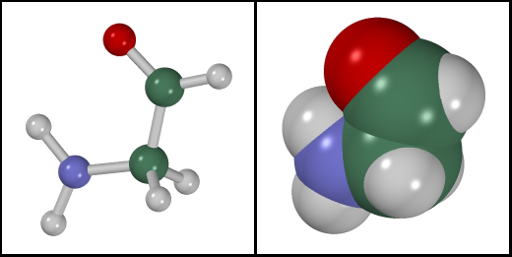
\includegraphics[width=100mm]{ball_cpk}
  \end{center}
  \caption{Ball-and-stick (left) and CPK (right) representations of the same
  molecule.}
  \label{fig:background_ball_cpk}
\end{figure}

% }}}

\paragraph{Solvent accessible surfaces}
% {{{

Solvent accessible surfaces \citep{connolly83} produces a similar effect to
CPK. The bonds are not visible and the atoms are enlarged, the difference lies
in the approach taken to produce the surface of the volume. The solvent
accessible surface is created by determining where the solvent (modelled using
spheres) can and cannot fit.

Figure \ref{fig:background_sas} is a schematic diagram illustrating how the
solvent accessible surface is determined. The molecular surface is marked in
purple. Even though the surface of the molecule (CPK representation) has many
crevasses, the solvent (the circles labelled with an `S') cannot fit in them and
thus the boundary is extended to where the solvent can fit.

\begin{figure}
  \begin{center}
    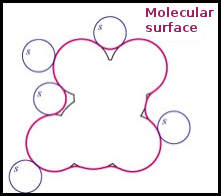
\includegraphics[width=60mm]{sas_ms}
  \end{center}
  \caption{Schematic diagram illustrating solvent accessible surfaces.}
  \label{fig:background_sas}
\end{figure}
% }}}

\paragraph{Protein molecules}
% {{{

The ribbon model (\citep{richardson81}, \citep{carson87}) was designed to
highlight the structure of protein molecules by fitting a curved surface to the
backbone of the molecule. This allows for the shape of the protein molecule to
be easily seen and followed.

Figure \ref{fig:background_ribbon} shows the backbone of a protein, the oxygen
atoms of the protein backbone are used to determine the normal for drawing the
oriented ribbon.

This has proved to be highly effective at highlighting the structure of
proteins. Unfortunately, this approach is not as effective when applied to
non-protein molecules such as carbohydrates and lipids, where the molecular
structure is different. Thus, the traditional ball-and-stick and CPK models are
still widely used for carbohydrate and lipid visualisation.

\begin{figure}
  \begin{center}
    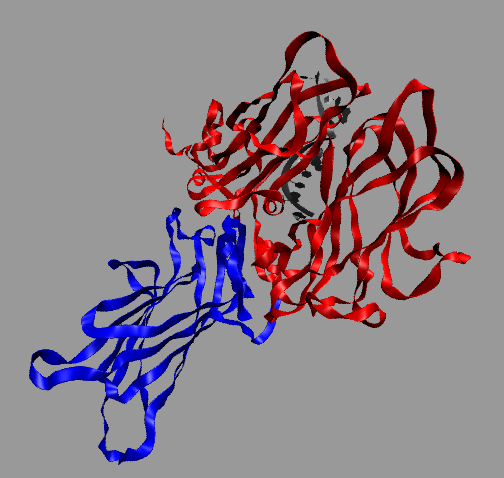
\includegraphics[width=60mm]{ribbon}
  \end{center}
  \caption{Ribbon model of a protein.}
  \label{fig:background_ribbon}
\end{figure}

% }}}

\paragraph{Carbohydrate molecules}
% {{{

The paper chain visualisation technique \citep{kuttel06} focuses on
highlighting ring structures in carbohydrate molecules. Ring structures are
first identified and are then displayed using a ring polyhedron.

This significantly simplifies the carbohydrate molecules by only showing the
carbohydrate rings, which would otherwise have been obscured in other
visualisations (ball-and-stick and CPK). The ball-and-stick model can still be
overlayed on the paper chain view to provide detailed information if needed.

The twister visualisation technique \citep{kuttel06} builds on the paper chain
technique by highlighting the relative orientations of the identified
carbohydrate rings. Each carbohydrate ring is represented by a disc, which is
then connected to another disc with a ribbon. The ribbon follows the
orientation from one ring to another, thus showing how the rings are connected
to one another.

The twister visualisation technique is similar to the ribbon model for proteins
in that it shows the overall shape of the molecule quite effectively. And, as
with the ribbon model, this visualisation technique is designed for a specific
type of molecule.

Figure \ref{fig:background_chain_twister} shows the paper chain and twister
models. The respective ball-and-stick representations of the carbohydrates are
overlayed semi-transparently over the models.

\begin{figure}
  \begin{center}
    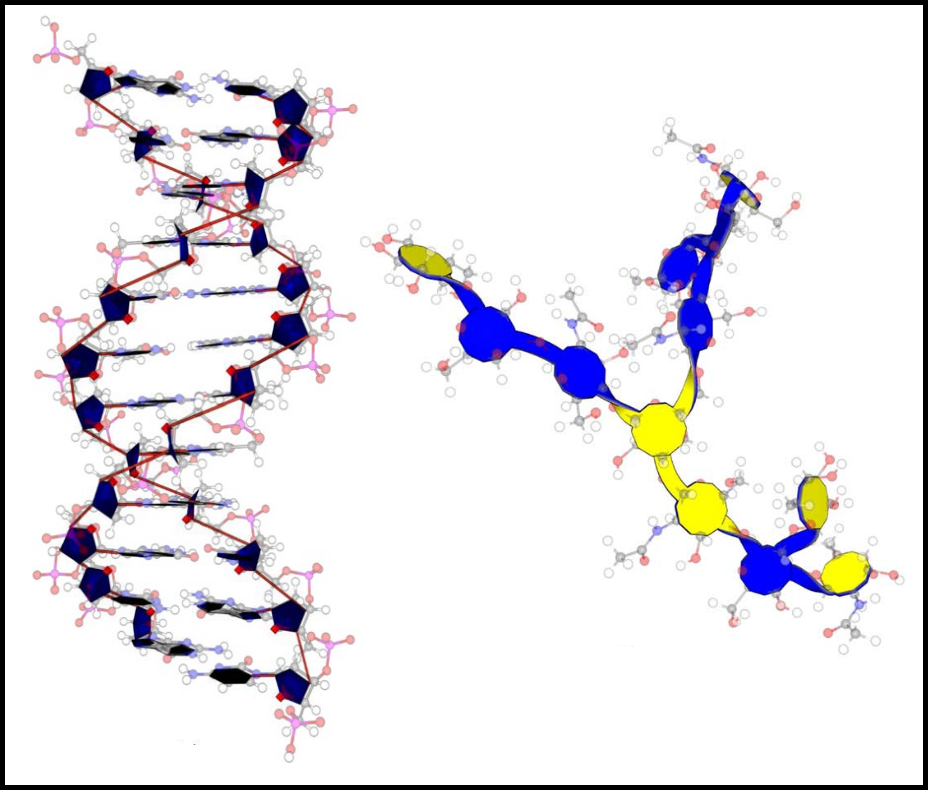
\includegraphics[width=100mm]{chain_twister}
  \end{center}
  \caption{Paper chain (left) and Twister model (right) of a carbohydrate, with
  ball-and-stick model overlayed semi-transparently.}
  \label{fig:background_chain_twister}
\end{figure}

% }}}

\paragraph{Summary}
% {{{

The different visualisation techniques discussed in this section are summarised
in Table \ref{tab:background_molecular}. The ball-and-stick representation is
used as the baseline for comparing against the other techniques. The table
lists the different molecular visualisation techniques, indicates the molecule
type that they are specific to, and whether they summarise the structure of the
molecule or not.

\begin{table}
  \begin{tabular}{ | l | l | l | }
  \hline
  Technique                   & Molecule type & Summarisation of structure?  \\ \hline
  Ball-and-stick              & All           &                              \\ \hline
  CPK                         & All           & A little                     \\ \hline
  Solvent accessible surfaces & All           & A little                     \\ \hline
  Ribbon                      & Protein       & Yes                          \\ \hline
  Paper chain                 & Carbohydrate  & Yes                          \\ \hline
  Twister                     & Carbohydrate  & Yes                          \\ \hline
  \end{tabular}
  \caption{Table summarising the molecular visualisation techniques, what
  molecule types they are specific to and do they summarise the structure.}
  \label{tab:background_molecular}
\end{table}

% }}}

% }}}

\section{General visualisation}
% {{{
\label{sec:background_general}

% {{{

The more relevant techniques from general visualisation with regards to point
cloud data are: surface extraction, volume rendering and general clutter
control techniques. Mesh decimation and metaballs are also relevant, but they
have more specific uses.

% }}}

\paragraph{Surface extraction}
% {{{

The marching cubes algorithm \citep{lorensen87} is the classical approach for
surface extraction. The algorithm works by sampling a 3D volume (voxelising the
volume) and then examining each voxel in the data to determine whether it is
inside the volume or not. A surface can then be determined by combining all the
voxels which intersect with the volume boundary. Figure
\ref{fig:background_mesh} shows the extracted surface of a skull.

Marching tetrahedrons is an alternative surface extraction algorithm to
marching cubes. Instead of using a cube as the sampling structure, a
tetrahedron is used. Each voxel in the data is split into 6 tetrahedrons, which
are used to determine whether that voxel intersects with the volume boundary.

Surface extraction allows for the shape of the volume to be extracted and
visualised, and is somewhat analogous to the CPK model in that regard. It can
be adapted to molecular data to provide a simpler, smoothed view of the
molecule, thus allowing for shape and contours to be more easily seen; which
may have otherwise been obscured by the details of the atoms.

The granularity of the sampling grid has a large impact on the quality of the
extracted surface. A grid where each individual voxel is quite small will
produce a detailed surface, but will correspondingly produce a large number of
polygons but these can be simplified away by mesh simplification. Section
\ref{sec:background_decimation} provides more detail on reducing the number of
polygons used to represent a surface.

\begin{figure}
  \begin{center}
    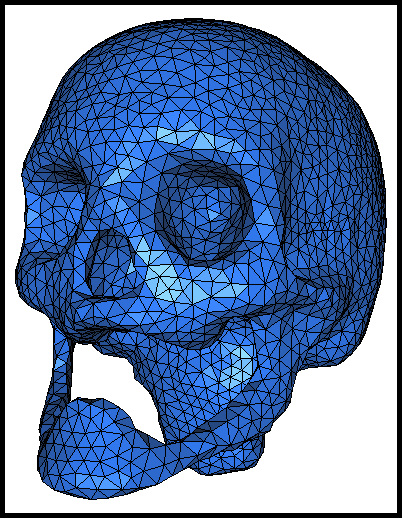
\includegraphics[width=50mm]{surface_mesh}
  \end{center}
  \caption{Extracted surface of a skull.}
  \label{fig:background_mesh}
\end{figure}

% }}}

\paragraph{Volume rendering}
% {{{

Volume rendering aims to visualise the entire volume instead of an object's
surface. The data is modelled as a translucent gel where one is able to see
through the volume, while still being able to see what is inside the volume.
Figure \ref{fig:background_head} is a ray cast image of a head. The internal
bones are clearly visible through the translucent skin and flesh.

There are two main approaches to volume rendering. The first works from the
image plane to the volume, and is called image order processing. Ray casting is
the typical approach to this problem as proposed by Levoy \citep{levoy88}. The
second approach, object order processing works from the volume to the image
plane. The classical approach to this is splatting \citep{westover89}. Hybrid
methods have been developed to take advantage of both approaches.

The main advantage of volume rendering is the ability to visualise the entire
volume at once, but this demands increased complexity and computation. Volume
rendering is not directly applicable to molecular data, but it can provide an
aggregated view of the entire volume.

\begin{figure}
  \begin{center}
    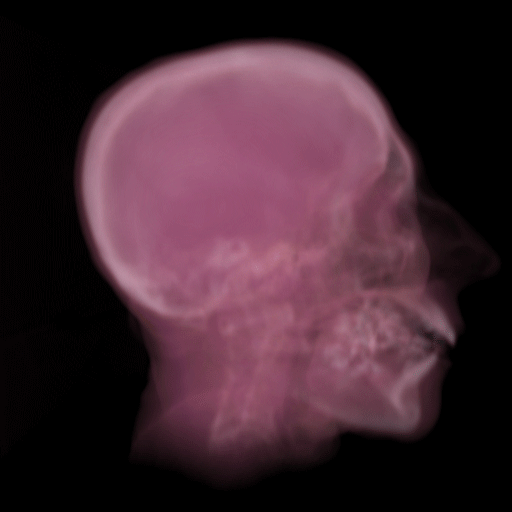
\includegraphics[width=70mm]{head_volume}
  \end{center}
  \caption{Ray cast image of a head.}
  \label{fig:background_head}
\end{figure}

% }}}

\paragraph{Clutter reduction}
% {{{
\label{sub:background_clutter}

Shneiderman provides a \emph{visual information-seeking mantra}
\citep{shneiderman96}: ``overview first, zoom and filter, then details on
demand'', which allows the consideration of clutter reduction techniques. The
methodology provides a general hierarchy of tasks to be applied to information
visualisation, in which clutter reduction plays an important role.

Ellis and Dix \citep{ellis07} provides a taxonomy cross referencing clutter
reduction techniques against certain criteria. With clutter reduction, a
trade-off between removing too much and too little information must be made.
Removing too much or too little data will produce a visualisation that is of
little use.

With regards to visualising point cloud data, \emph{filtering} \citep{stone94},
\emph{opacity} \citep{kosara02} and \emph{topological distortion}
\citep{lamping96} are the most useful clutter reduction techniques.

\emph{Filtering:} Only certain objects fulfilling certain criteria are
displayed in order to reduce clutter. The criteria can consider certain
characteristics or objects in a certain area or locus of interest; irrelevant
objects are removed. Uninteresting occluding objects are also removed to show
objects in important areas or with important characteristics.

Another approach to filtering is to highlight the important features of the
data with colour, but leave the rest of the data visibly unchanged. This has
the advantage of maintaining context.

Figure \ref{fig:background_highlight} is an example application of highlighting
in a graph structure. The more oftenly traversed paths are more important,
which is reflected in the colouring. From looking at the image, it is clear
that the intersection on the right edge of the image is the most heavily
traversed area of the graph as it is the brightest.

\emph{Opacity:} The translucency of items can be changed to highlight or hide
elements. This is similar to filtering, in that irrelevant items are partially
or entirely hidden, highlighting only the important parts. The advantage of
opacity over filtering is that other information is not entirely removed, it is
still available if needed and can be used to hint at contextual information.
Opacity can also be adapted to show temporal information, where the previous
frame is rendered along with the current frame, but at a lower opacity;
creating an effect similar to motion blur.

\emph{Topological distortion:} The representation of the data can be changed so
that certain areas are larger. This highlights and focuses on the relevant
areas, while de-emphasising the other areas. The distortion can either be
uniform (zooming), or can be non-uniform (fish-eye effect).

Clutter reduction techniques have the most potential for point cloud
visualisation as there is a need to be able to visualise many objects in 3D
space. However, care must be taken to not remove important and relevant
information. It should be noted that clutter reduction techniques are not all
mutually exclusive, many of the techniques complement one another.

\begin{figure}
  \begin{center}
    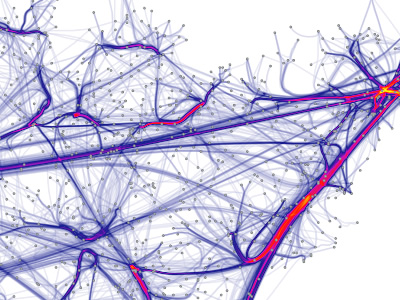
\includegraphics[width=70mm]{graph_highlight}
  \end{center}
  \caption{Colour is used to highlight highly traversed path.}
  \label{fig:background_highlight}
\end{figure}

% }}}

\paragraph{Metaballs}
% {{{

Metaballs \citep{blinn82} is a technique for producing organic-looking objects.
The metaballs volume is modelled using a number of points that exert forces
around themselves, the surface of the volume is determined by the set of points
where the force function is equal to some constant threshold value. The surface
is usually determined using surface extraction techniques.

There are 15 metaball points in Figure \ref{fig:background_metaballs}, the
metaball points are the roundish parts of the volume. Areas of the volume
appears to melt and blend together, yielding the blobbly appearance. The force
functions used takes into account the nearby metaball points, which causes the
merging effect.

The advantage of metaballs is that volume data is grouped together, making it
easy to see the different volumes in a region. The disadvantage of this
technique is the computational cost required to determine and extract the
surface from the force calculations.

\begin{figure}
  \begin{center}
    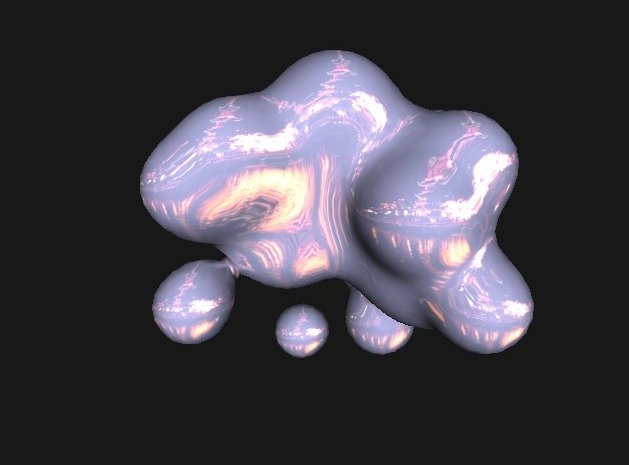
\includegraphics[width=70mm]{metaballs}
  \end{center}

  \caption{A volume determined with 15 metaballs exerting forces around
  themselves.}

  \label{fig:background_metaballs}
\end{figure}

% }}}

% }}}

\section{Mesh decimation}
% {{{
\label{sec:background_decimation}

The amount of time taken to render a model is proportional to the number of
polygons in the model. There is thus a trade-off between detail and render
time: more polygons will increase the amount of detail present, but will also
increase render time. Mesh decimation is a technique aimed at reducing the
number of polygons used to represent a mesh while preserving as much detail as
possible.

Mesh decimation can be broadly divided into two main categories:
\emph{geometric decimation} and \emph{vertex clustering}. A more complete
comparison between mesh simplification algorithms can be found in Cignoni et
al. \citep{cignoni98}.

\paragraph{Geometric decimation}
% {{{

Geometric decimation iteratively eliminates components of the mesh: vertices,
edges or faces \citep{schroeder92}. The component to be removed is chosen using
local geometric optimality criteria. After eliminating the component, a local
re-triangulation process is used to fill in any resulting holes.

% }}}

\paragraph{Vertex clustering}
% {{{

Vertex clustering groups a number of geometrically similar and spatially close
vertices together \citep{rossignac93}, the group of vertices is then replaced
by a new representative vertex. Due to the simplicity of the test, vertex
clustering can be implemented very efficiently.

% }}}

% }}}

\section{Summary}
% {{{
\label{sec:background_summary}

This chapter has presented some visualisation techniques, each with their own
advantages and disadvantages. Visualisation techniques are best designed to
take advantage of specific domain knowledge. As a result, they are not easily
generalisable into other areas.

Molecular modelling is a specific instance of the scientific visualisation
problem, where the requirement is to be able to easily identify certain
structures. Different types of molecules each have their own specific
characteristics and structures. This knowledge can be exploited in the
different visualisation techniques: the ribbon representation is useful for
proteins, paper chain and twister for carbohydrates, while ball-and-stick and
CPK for general molecular visualisations.

General visualisation techniques address a slightly different problem: how to
visualise the data effectively and not necessarily to identify and highlight
specific structures. Thus the main concern is how to enable easy exploration of
the data.

None of the techniques touched on, handle time explicitly. If a temporal
dimension were to be added, all the techniques would simply treat each frame
separately and regenerate the visualisation given the new set of data. This
approach is not ideal if some interframe visualisation coherence is desired.

Visualising point cloud data, where there are many points in a region, is also
not very well handled. With water visualisation, the points are distributed
within a three dimensional volume, which makes visualisation more difficult.

There is no single solution for all visualisation needs. However, approaches
and ideas can be taken from different visualisation approaches. While the
problems may not be identical, there will be some overlapping requirements and
concerns.

% }}}

% }}}


\graphicspath{{./design/}}

\chapter{Design}
% {{{
\label{cha:design}

% {{{

The goal of the visualisation aspect of the system is to provide a way to
easily interpret the molecular data. The visualisation techniques chosen either
support the compression aspect of the water compression system, or allows for
general interpretation of data. The main challenge to the effective
visualisation of the data is the large amounts of visible clutter.

A brief overview of the entire system is provided in Section
\ref{sec:design_overview}, while Section \ref{sec:design_visualisation} provides
more detail into the visualisation components of the system.

% }}}

\section{System overview}
% {{{
\label{sec:design_overview}

The design of the system has been broken down into a number of components. The
most notable components are:

\begin{itemize}
  \item Quantiser - quantises and dequantises the data
  \item I/O - handles input and output of data
  \item Water cluster extractor - extracts the water clusters
  \item Verifiers - verify and record various aspects of the compression system
  \item Arithmetic coders - encodes and decodes symbols
  \item Visualisation - displays the simulation data
  \item Compressors - drivers behind the compression system
\end{itemize}

See Figure \ref{fig:design_overview} for a schematic diagram of the components
listed above. Julian Kenwood has completed the green areas, Keegan Smith has
completed the cyan areas, while I have completed the red areas. The Quantiser,
I/O and Water cluster extractor components are used by both the compressors and
the visualisation. The Verifiers and Arithmetic coder components are used by the
compressors only.

\begin{figure}[h!]
  \begin{center}
    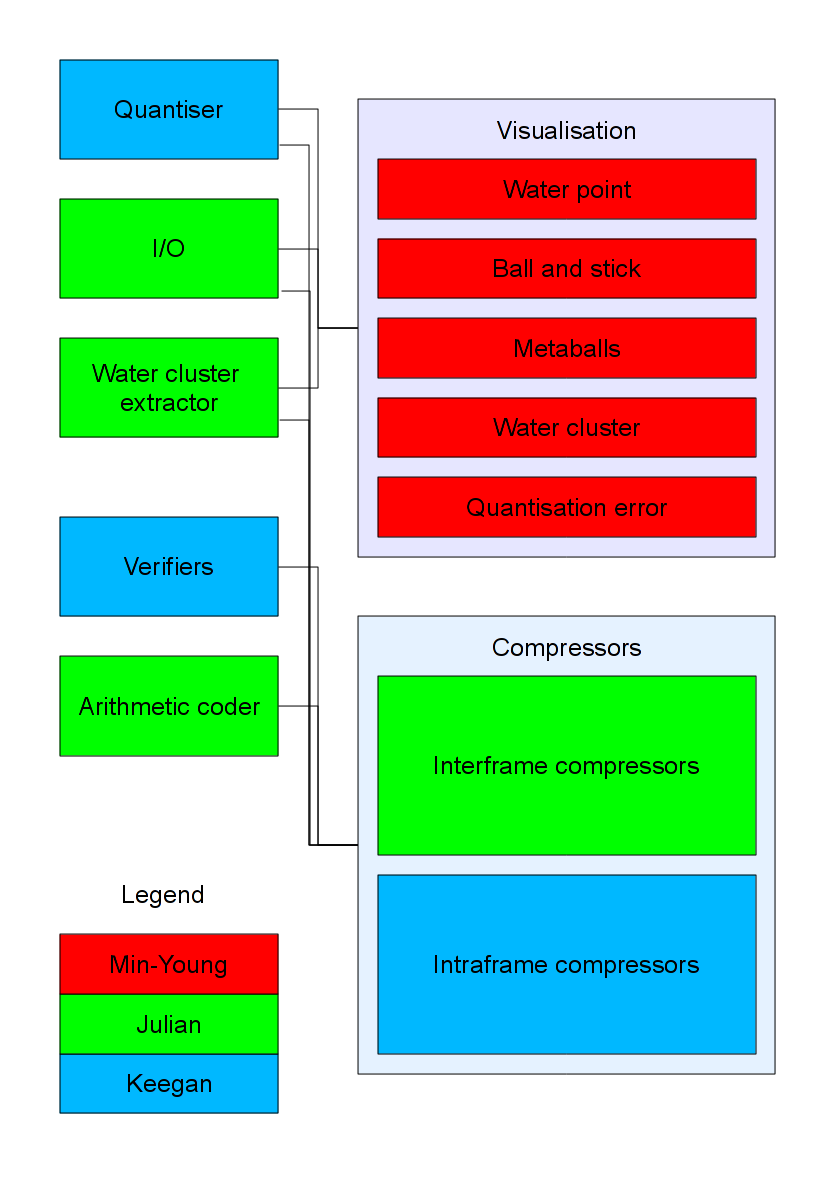
\includegraphics[width=100mm]{breakdown}
  \end{center}
  \caption{Overview of components within the system}
  \label{fig:design_overview}
\end{figure}

% }}}

\section{Visualisation}
% {{{
\label{sec:design_visualisation}

% {{{

The visualisation component is divided into a number of sub-components, which
are the different visualisation techniques chosen:

\begin{itemize}
  \item Water point visualisation
  \item Ball and Stick visualisation
  \item Metaballs visualisation
  \item Water cluster visualisation
  \item Quantisation error visualisation
\end{itemize}

% }}}

\subsection{Water point visualisation}
% {{{
\label{sub:design_waterpoint}

This visualisation technique is the simplest of all the visualisation
techniques in the system. A single point will be rendered per water molecule,
non-water molecules will be filtered out. Filtering out the non-water molecules
is the first step in reducing visible clutter. Using a low alpha value per
point further reduces clutter by causing areas with few overlapping points to
be more less visible, in comparison to areas with many overlapping points;
hence emphasising the areas with many overlapping points.

The advantage of this visualisation technique is that it allows for the larger
areas of water to be easily identified, however, the details are hidden.

% }}}

\subsection{Ball and stick visualisation}
% {{{
\label{sub:design_ballstick}

The ball and stick visualisation technique is used to provide more visual
information about the water molecules, the individual atoms of the water
molecules are visible. Rendering the individual atoms allows for the
orientation the water molecules to be seen.

As rendering all the water molecules will cause much clutter, the number of
molecules to render can be limited.

% }}}

\subsection{Metaballs visualisation}
% {{{
\label{sub:design_metaballs}

The metaballs technique is an alternative way to visualise the water volume in
the molecular simulation. The aim of the metaballs technique is to clearly
separate the areas of water, from the non-water areas. A surface is rendered
between the water and non-water areas of the volume.

To decrease the rendering cost of the surface, the surface is decimated.
Decimating the surface will simplify the surface, hence decrease the time
required to render it, and allow the volume to be more easily explored.

An alternative to decimating the surface in order to decrease the surface
complexity, is to decrease the amount of sampling done. Sampling the volume
less results in fewer triangles, but the surface quality will also decrease.

Decimation is preferred to decreasing the sampling amount as the surface
quality can be maintained. The render cost is decreased in exchange for
computation cost, where the computation is performed once for every frame.

% }}}

\subsection{Water cluster visualisation}
% {{{
\label{sub:design_watercluster}

The water molecules in a body of water is not completely uniform in all
directions, instead the water molecules form clusters. The compressors use this
knowledge to perform prediction, and thus it is useful to visualise these water
clusters.

To cope with the large number of water clusters that are present, the number of
clusters to render can be limited. Specific water clusters can also be rendered.

This visualisation technique is primarily useful in supporting the compression
aspect of the system. There has not been much emphasis on water clusters in
chemistry, thus it is unlikely that this visualisation technique will be of
interest to chemists.

% }}}

\subsection{Quantisation error visualisation}
% {{{
\label{sub:design_quanterror}

Quantisation is the only lossy step of the compression, thus it is important to
measure the amount of error that is introduced. To visually depict the
quantisation errors, the water molecules are coloured according to a colour
gradient. Water molecules with high quantisation errors are coloured so that
they are more visible and stand out, while water molecules with low
quantisation errors will be less visible.

This visualisation technique is only useful in supporting the compression aspect
of the system.

% }}}

% }}}

% }}}


\graphicspath{{./implementation/}}

\chapter{Implementation}
% {{{
\label{cha:implementation}

The implementation details of the program are discussed in this chapter.

Section \ref{sec:implementation_details} details the platform, language and
libraries choices of the program. Section \ref{sec:implementation_techniques}
provides implementation details on each of the visualisation techniques.
Section \ref{sec:implementation_limitations} identifies the limitations and
short-comings of the visualisation approaches.

\section{Details}
% {{{
\label{sec:implementation_details}

\paragraph{Linux}
% {{{

Due to the large number of freely available libraries for Linux, this was
chosen as the preferred platform for development.

% }}}

\paragraph{C++}
% {{{

To ensure easy interoperability between the different components of the system,
it was decided that the same language be used for all the components. The
compression aspect of the system requires efficient access to memory and usage
of the CPU; therefore C++ was the logical choice of programming language. As
such, C++ is the programming language used throughout the system.

% }}}

\paragraph{Qt}
% {{{

The cross platform Qt widget library \citep{Qt} was used to produce the user
interface for the visualisation program. While there are numerous other
alternatives to Qt, GTK+ being the next best alternative, Qt provides the
richest development framework, hence making it the easiest to use.

% }}}

\paragraph{OpenGL}
% {{{

To visualise the molecular data in real time, hardware accelerated graphics is
needed. Thus, OpenGL \citep{OpenGL} was employed to produce the graphics for
the visualisation. A software renderer would not be able to produce the scenes
as fast as a graphics processor would. OpenGL is preferred over DirectX due to
the following considerations: it is cross platform, Qt has support for an
OpenGL widget, and DirectX is not available on Linux.

% }}}

\paragraph{GTS}
% {{{

Due to difficulties encountered in decimating the surfaces generated for the
metaballs visualisation, a library is used to decimate the surface instead of
reproducing a decimation algorithm. The library used is the GNU Triangulated
Surface Library \citep{GTS}. The library uses the decimation algorithm proposed
by Lindstrom and Turk \citep{lindstrom98}.

% }}}

\paragraph{Licensing}
% {{{

All the libraries used directly by the visualisation program (Qt and GTS) are
licensed under the LGPL \citep{LGPL}, which means that any program can freely
link against and use these libraries. There are no restrictions placed on the
visualisation component of the system by the libraries used.

% }}}

% }}}

\section{Visualisation Techniques}
% {{{
\label{sec:implementation_techniques}

\subsection*{Water point}
% {{{

The water point visualisation renders a single OpenGL point primitive for each
water molecule. All the points drawn have a very low alpha value; so that the
colour at a point will become more intense as more points overlap.

An effective alpha value and point size will depend on the molecular data: how
dense the water molecules are. If the water molecules are not very dense, then
a higher alpha value will be needed to make the individual points visible. For
densely populated volumes, a lower alpha value can be used.

Point size has a similar effect as alpha value: a larger point size will result
in more overlapping points, hence causing the colour intensity to increase more
quickly. For less dense volumes, the point size should be larger so as to
increase its effect on the output. More densely populated volumes should use
smaller points sizes to avoid reaching the maximum intensity value.

Figure \ref{fig:implementation_waterpoint} shows the water point visualisation.
There are two separate regions on water in the data, this is reflected in the
figure by the left and right areas of blue. There is a region of non-water in
the middle. The same dataset is used for all the images in this chapter so that
the different visualisation can be compared.

\begin{figure}
  \begin{center}
    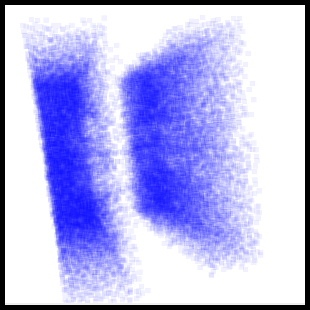
\includegraphics[width=50mm]{waterpoint}
  \end{center}
  \caption{Water point visualisation. Each point represents a water molecule.}
  \label{fig:implementation_waterpoint}
\end{figure}

% }}}

\subsection*{Ball-and-stick}
% {{{

The colour and size of the spheres used to represent the oxygen and hydrogen
atoms are configurable. Similarly, the cylinder size and colour representing
the bonds can be configured. By changing the sphere sizes, the ball-and-stick
visualisation technique can be made to mimic the CPK approach.

Lighting can be enabled to better see the spheres.

Figure \ref{fig:implementation_ballstick} shows some water molecules rendered
using the ball-and-stick visualisation technique. The red spheres represent
oxygen atoms, while the blue spheres represent hydrogen atoms. The
left image uses the classical approach, where cylinders are used to connect the
atoms together. The right image uses the CPK approach, where the atoms are
enlarged to encompass the molecular bond.

\begin{figure}
  \begin{center}
    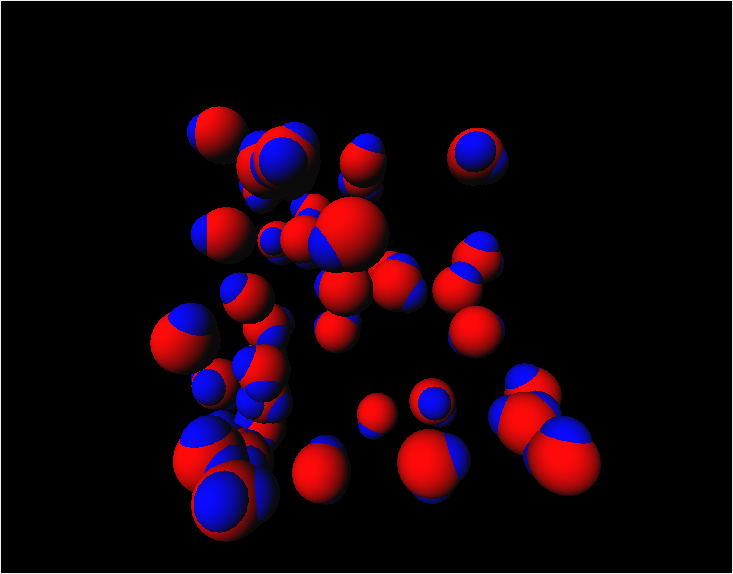
\includegraphics[width=100mm]{ballstick}
  \end{center}
  \caption{Ball-and-stick visualisation. The left image uses the classical
  approach, while the right image uses the CPK approach.}
  \label{fig:implementation_ballstick}
\end{figure}

% }}}

\subsection*{Metaballs}
% {{{

Due to the large number of water molecules, performing a na\"ive comparison
against all the water molecules is very inefficient. Instead, a grid is used to
place the water molecules and test for whether a point is inside or outside a
region of water.

The step size for sampling the volume and the threshold value to use in
determining the surface can all be configured in the user interface. The
threshold value is the main determinant in what the output surface looks like.

% {{{

For the metaballs visualisation technique, a surface needs to be extracted; the
marching cubes and marching tetrahedrons surface extraction algorithms were
both implemented. The algorithms were compared to one another to determine
which algorithm is preferred. The various aspects compared were:

\begin{itemize}

  \item Time for surface extraction - time required to extract the surfaces
  from the volume data.

  \item Surface primitive count - number of surface primitives generated for
  the volume.

  \item Surface quality - the extracted surfaces are visually compared for
  noticeable differences.

\end{itemize}

The two algorithms were tested on the datasets used for the quantisation
experiment (Chapter \ref{cha:experiment}).

Table \ref{tab:appendix_surface_time} in Appendix \ref{cha:tables}, shows the
time required for extracting the surfaces from the volume data. The results
indicate that marching tetrahedrons requires more time to extract the surface,
the extra time required ranges from 50 to 800 milliseconds more. The extra time
required is not considerably large, but the difference is noticeable.

Table \ref{tab:appendix_surface_count} in Appendix \ref{cha:tables}, shows the
number of surface primitives in the extracted surfaces. The surfaces extracted
by marching tetrahedrons are all composed of at least twice as many surface
primitives as that extracted by marching cubes. The extra surface primitives
will increase rendering cost, as well as time required for decimation. This is
the largest factor used in preferring marching cubes over marching
tetrahedrons.

Figure \ref{fig:implementation_compare} shows the surface extracted from
marching cubes on the left, and the surface extracted by marching tetrahedrons
on the right. The view has been zoomed in to more clearly see the surface
differences. The visual differences between the extracted surfaces are minor,
especially when the view is zoomed out to view the entire volume.

\begin{figure}
  \begin{center}
    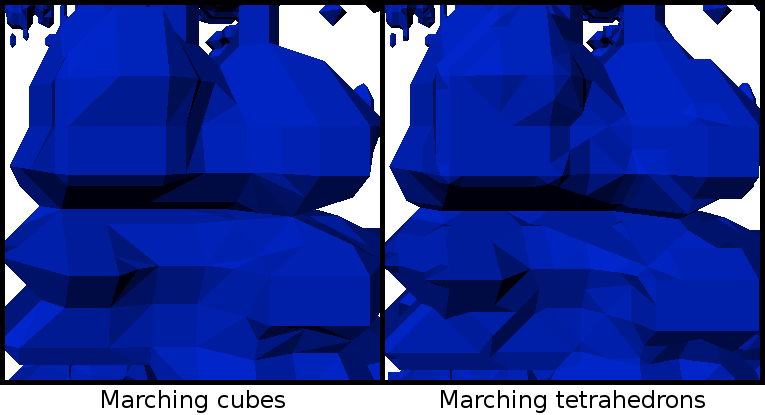
\includegraphics[width=100mm]{surface_compare}
  \end{center}
  \caption{Surface generated by marching cubes (left) and marching tetrahedrons
  (right).}
  \label{fig:implementation_compare}
\end{figure}

As the surface differences are minor, the algorithm that produces fewer
triangles is preferred, which is marching cubes.

% }}}

% {{{

As was mentioned in Section \ref{sec:implementation_details}, the GTS library
is used to perform the surface decimation. Due to unforeseen difficulties and
time constraints, using a library was the fastest way to achieve decimation.

The computational cost for a single frame in the metaballs visualisation is
quite high. A frame can only be generated in real time for small volumes (less
than 500 water molecules). Larger volumes may take upwards of 5 seconds or more
for a single frame to be generated. Performing decimation on the extracted
surface will only increase the computational cost. A pre-processing option is
thus available. All the frames can be pre-processed and saved to file. The
output file is a simple dump of the vertices and normals of all the triangles.
This file can then be used to render the surface without the processing
overhead.

When rendering the surface, one side of the surface is coloured blue, while the
other is coloured green. This allows differentiation of the different sides of
the surface. The blue side of the surface is facing the non-water area of the
volume, while the green side of the surface is facing towards the water area.

Figure \ref{fig:implementation_metaballs} shows the metaballs visualisation for
the data used for Figure \ref{fig:implementation_waterpoint}. The large green
surface on the left part of the figure faces into the left region of water,
behind the surface is a region of non-water. The large blue surface on the
right is the boundary between the region of non-water in the middle, and the
region of water to the right. There are some smaller surfaces in the left and
right areas, which further defines the regions of water.

To help see the surface detail, lighting can be enabled.

\begin{figure}
  \begin{center}
    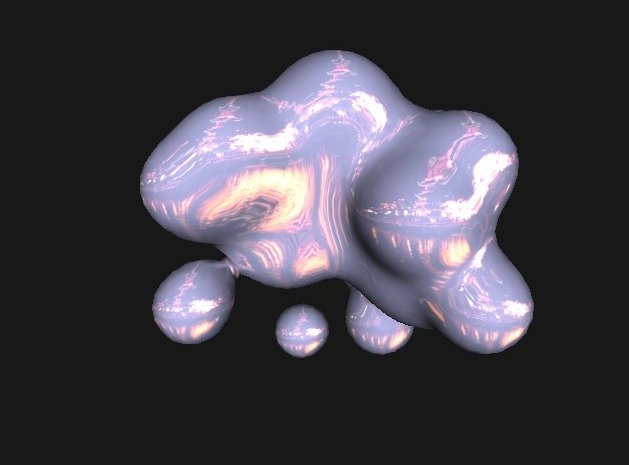
\includegraphics[width=50mm]{metaballs}
  \end{center}
  \caption{Metaballs visualisation. Renders the surface between water and
  non-water molecules.}
  \label{fig:implementation_metaballs}
\end{figure}

% }}}

% }}}

\subsection*{Water cluster}
% {{{

The colour and size of the cylinders used to connect the water molecules
together are all configurable in the user interface.

Lighting can be enabled for this visualisation technique so that the shape and
orientation of the cylinders can be more easily determined.

Figure \ref{fig:implementation_watercluster} shows the water cluster
visualisation where three water clusters are visible. The extracted water
clusters are often quite small, mostly consisting of a few water molecules only.

\begin{figure}
  \begin{center}
    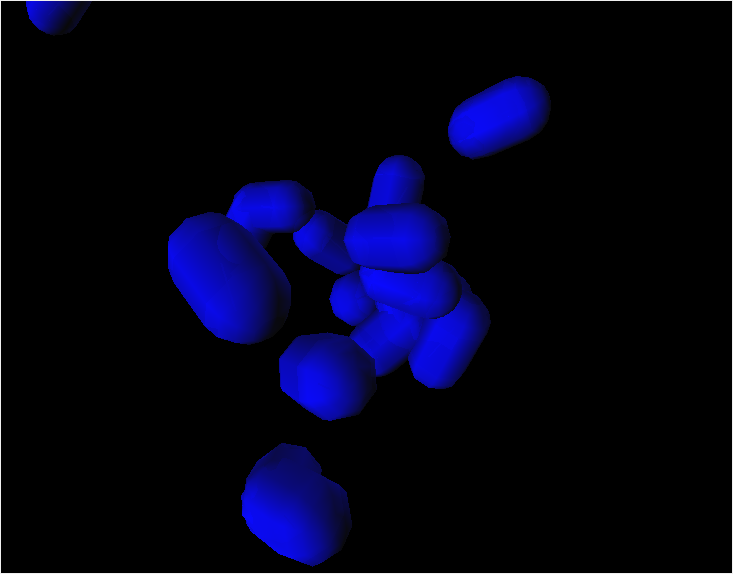
\includegraphics[width=50mm]{watercluster}
  \end{center}
  \caption{Water cluster visualisation. Water molecules within cluster are
  joined using cylinders.}
  \label{fig:implementation_watercluster}
\end{figure}

% }}}

\subsection*{Quantisation error}
% {{{

The starting and final error colours and values are all configurable from
within the user interface.

Figure \ref{fig:implementation_quanterror} shows the quantisation errors for
the example volume used in this chapter. The point rendering (left) and line
rendering (right) modes are shown in the figure. The point rendering renders a
point for the water molecule, while the line rendering renders a line between
the original and quantised positions.

The red areas indicate large quantisation error, while the fainter green areas
indicate lower quantisation error. Due to the stepped colour scale, the
different areas are clearly visible.

\begin{figure}
  \begin{center}
    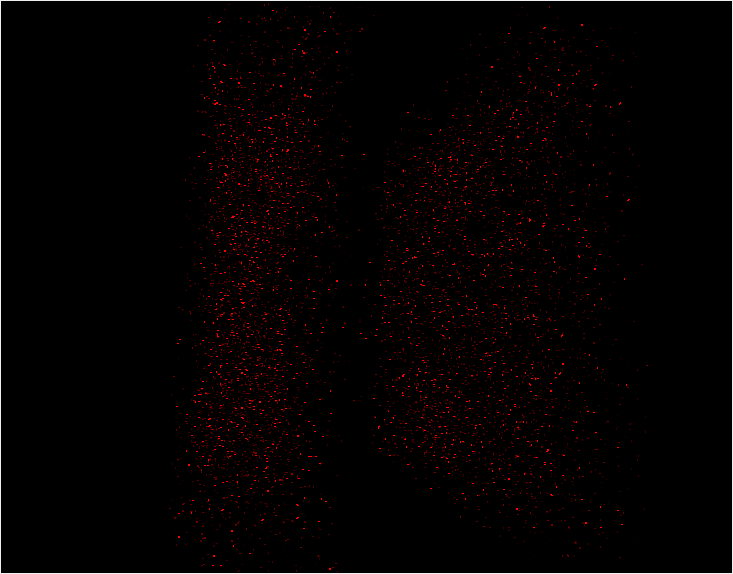
\includegraphics[width=120mm]{quanterror}
  \end{center}
  \caption{Quantisation error visualisation. Quantisation errors are visualised
  using either points (left) or lines (right).}
  \label{fig:implementation_quanterror}
\end{figure}

% }}}

% }}}

\section{Limitations}
% {{{
\label{sec:implementation_limitations}

As the data can be very different, some adjustments to various configuration
values will need to be made to most effectively visualise the data. An example
of such a change is the alpha value and point size for the water point
visualisation technique. For small volumes, a high alpha value and point size
will be needed to effectively visualise the volume. Other changes will need to
be made for the other visualisation techniques. These changes are unfortunately
unavoidable.

The water point visualisation technique is only useful for volumes where there
are large amounts of water and non-water. If the volume is small or uniformly
filled with water molecules, the alpha effects will not be significant.

The metaballs visualisation technique requires considerable processing for each
frame (surface extraction and decimation), hence real time rendering is only
possible for small volumes. The amount of rendering time required is dependant
on the number of water molecules and extracted surface, processing time for a
single frame can be from a few seconds, up to a minute. Disabling decimation
will decrease the time required for a single frame, processing time then ranges
from a few hundred milliseconds, up to 10 seconds.

There is an option to pre-process the volume and save the extracted surfaces to
file, however, the generated files are generally considerably larger than the
DCD file. The size of the pre-processed file is dependant on the number of
water molecules and number of frames. From the data used for the quantisation
experiment, the pre-processed file were an average of 10 times larger than the
DCD file. The smallest output file was the same size as the DCD file, while the
largest was 100 times larger.

To limit the file size and pre-processing time, the number of frames to
pre-process is limited. This number can be set by the user.

% }}}

% }}}


\graphicspath{{./experiment/}}

\chapter{Quantisation Experiment}
% {{{
\label{cha:experiment}

The position data to be compressed in our water compression system is stored as
floating point data. To facilitate compression, the floating point data is
converted to integer values through quantisation. An appropriate number of
bits, the range of integer values, needs to be decided. Fewer bits will result
in higher compression, but more quantisation error will be incurred; while more
bits will result in lower compression, but the data is stored more accurately.

To determine the appropriate level of quantisation, an experiment was conducted
to test the perceptually visible effects of quantisation. More simply stated:
how noticeable are the effects of quantisation? This will help determine the
appropriate level of quantisation; using the least number of bits, while
maintaining visual similarity to the original data.

\paragraph{The experiment hypothesis is:} what is the level of quantisation where the
perceived differences between the original and quantised data are not
significantly different.

The rest of this chapter details various aspects of the experiment.

\section{Introduction}
% {{{
\label{sec:experiment_introduction}

The participants in the experiment were required to rate the difference between
the original unquantised data, and the quantised data. They used a scale of 1
to 7 to rate the difference, 1 being ``Not different'' and 7 being ``Very
different''. Two different visualisation techniques, and four different
quantisation levels were tested. The experimental procedure is detailed in
Section \ref{sec:experiment_procedure}.

Figures \ref{fig:experiment_ballstick4680} and
\ref{fig:experiment_metaballs4680} show the different quantisation levels for
the ball-and-stick, and metaballs visualisation techniques, respectively. The
original unquantised data is on the left, with the four different quantisation
levels; 10 and 8 bit quantisation at the top, 6 and 4 bit quantisation at the
bottom.

\begin{figure}
  \begin{center}
    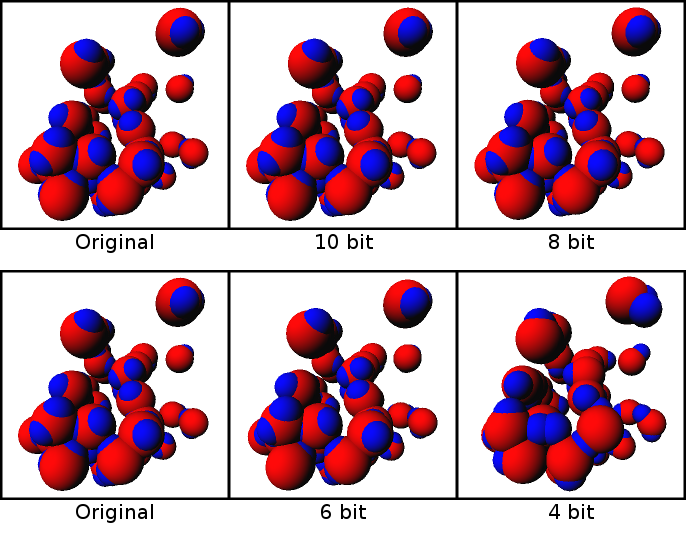
\includegraphics[width=120mm]{ballstick4680}
  \end{center}
  \caption{Ball-and-stick visualisation showing the different quantisation
  levels}
  \label{fig:experiment_ballstick4680}
\end{figure}

\begin{figure}
  \begin{center}
    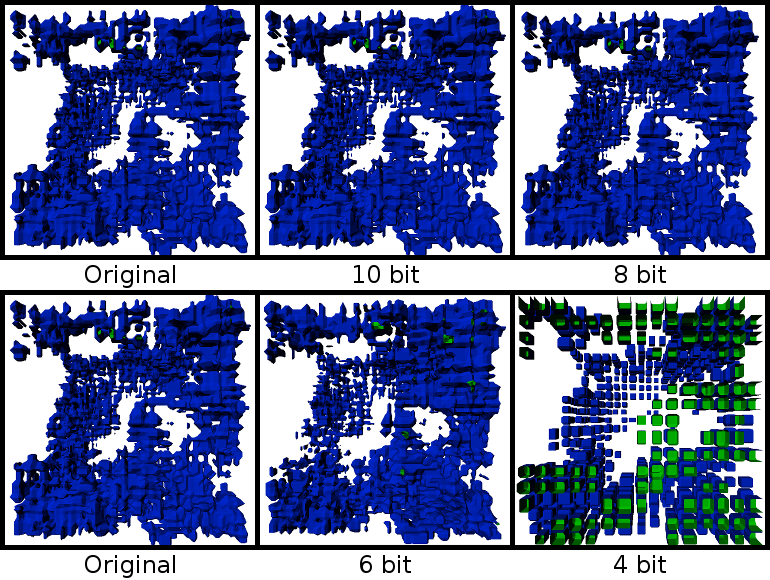
\includegraphics[width=120mm]{metaballs4680}
  \end{center}
  \caption{Metaballs visualisation showing the different quantisation
  levels}
  \label{fig:experiment_metaballs4680}
\end{figure}

% }}}

\section{Venue and equipment}
% {{{
\label{sec:experiment_venue}

The participants took part in the experiment one at a time within a closed
room. They watched the data on a 19-inch CRT monitor, which was connected to a
laptop. The laptop was used to load and display the data. The same laptop was
used for all the experiments: \begin{itemize} \item Processor: Intel Core 2 Duo
Processor T6570 2.1GHz \item Memory: 2GB DDR2 \item GPU: Mobile Intel Graphics
Media Accelerator X4500 HD \end{itemize}

% }}}

\section{Participants}
% {{{
\label{sec:experiment_participants}

All the participants were students from the University of Cape Town. Half of
the participants were Science students, with the remaining half consisting
mostly of Commerce and Humanities students. Nineteen of the participants were
male; the remaining 11 participants were female.

Only one of the participants has a significant background in chemistry, i.e.
studies chemistry. Inspecting her results indicates that they are similar to
all the other participants. As there is insufficient data, statistical analysis
cannot be reliably applied to determine if her responses were significantly
different. Her results were not removed from the analysis.

The only requirement for a participant to take part in the experiment was that
they not be visually impaired. This is called ``vision corrected to normal''
and is common in perceptual experiments. All that is needed is that they are
able to watch and compare two different sets of data (molecular
visualisations).

A total of 30 participants took part in the experiment. Most of the experiments
were completed in the first three days (25 of the planned 30), while the
remaining experiments were completed over three more days. A single session was
used for each participant.

% }}}

\section{Variables}
% {{{
\label{sec:experiment_variables}

The variables of the experiment are the four different quantisation levels, and
the two different visualisation techniques.

The four quantisation levels tested were: 4, 6, 8 and 10 bit quantisation.

10 bit quantisation was chosen as the upper quantisation level because beyond
this setting, the quantisation effects are too minimal to be noticeable as
determined by a pilot experiment. Even at 10 bit quantisation, the differences
are miniscule (see Figure \ref{fig:experiment_ballstick4680}).

The two visualisation techniques were: ball-and-stick, and metaballs.

At the time of the experiment, there were four datasets available, all of which
were used and randomly assigned to the participants.

% }}}

\section{Procedure}
% {{{
\label{sec:experiment_procedure}

The following experimental procedure was consistently applied to each of the
participants that took part in the experiment.

\begin{enumerate}

  \item The subject is given a piece of paper explaining the experiment and
  what they are required to do.

  \item A random dataset is selected for the participant.

  \item The original unquantised data is loaded and the subject is allowed to
  explore and view it.

  \item Thereafter, two different quantised data are loaded for the subject to
  view.

  \item The original data is loaded again to remind the participant what the
  original data looked like.

  \item A final two more quantised data are loaded.

  \item The quantisation levels are chosen in a random order.

  \item After showing each quantised data, the subject is asked to compare it
  with the original data, indicating on a scale of 1 to 7, how noticeable the
  differences are: 1 being ``Not different'' and 7 being ``Very different''.

  \item This procedure is repeated for a total of 2 visualisation techniques,
  with 2 different datasets each.

  \item The order of visualisation techniques shown is the same for all
  participants: first ball-and-stick, then metaballs.

\end{enumerate}

On average, the participants took 25 minutes to complete the experiment. The
duration of the experiment varied due to the different datasets. Not all
datasets were of equal size or length, some datasets required more time to play
from start to finish.

After conducting a pilot experiment, it was decided that the participants
should not be able to rotate and explore the data. Rotating the view makes the
data look very different and the participants might become lost and
disoriented. This could invalidate the results of the experiment as the
participants would not be able to accurately compare the unquantised and
quantised data. This becomes more a test of navigation than viewing and prior
experience would play a part.

% }}}

\section{Summary}
% {{{
\label{sec:experiment_summary}

The experiment used the ball-and-stick, and metaballs visualisation techniques;
with 4, 6, 8 and 10 bit quantisation levels. A total of 30 participants took
part in the experiment, each viewing two different datasets. There were four
datasets used in the experiment, thus, each dataset was viewed by 15
participants.

Over the four datasets, a total of 60 scores per quantisation level were
recorded. The results from the experiment are presented and analysed in Chapter
\ref{cha:results}.

% }}}

% }}}


\graphicspath{{./results/}}

\chapter{Results}
% {{{
\label{cha:results}

This chapter presents the results for the quantisation experiment. Section
\ref{sec:results_methodology} details the approach taken to analysing the
various data. Section \ref{sec:results_results} presents the results from
analysing the data. The results are discussed in Section
\ref{sec:results_discussion}. Finally, Section \ref{sec:results_summary}
summarises this chapter.

Data from the different datasets in the quantisation experiment is first
presented and analysed. Finally the data from the experiment is aggregated to
provide for a more general analysis on the perception of quantisation.

\section{Methodology}
% {{{
\label{sec:results_methodology}

To analyse the responses from the experiment, a series of statistical tests are
conducted on the data to determine various statistical properties.

\paragraph{Shapiro-Wilks Test}
The first test is for normality. Further tests conducted on the data depend on
whether the data is normal or not, thus it is important to determine the
normality of the data. The hypothesis and null hypothesis of the Shapiro-Wilks
Test are: \\ \\
\textbf{Hypothesis:} The data is a normal distribution. \\
\textbf{Null hypothesis:} The data is not a normal distribution.

\paragraph{Friedman Test}
Determining if the datasets have an impact on the perceived differences for a
specific quantisation level needs to be undertaken. However, we discovered that
some the dataset specific data does not form a normal distribution. Hence,
non-parametric statistical analysis will need to be conducted.

If the data is not normal, the Friedman Test can be used to determine if the
factors have a statistically significant impact on the data. For this
experiment, the hypothesis and null hypothesis are: \\ \\
\textbf{Hypothesis:} The datasets used have an impact on the results. \\
\textbf{Null hypothesis:} The datasets do not have impact on the results.

\paragraph{ANOVA}
The aggregated data for the different quantisation levels and visualisation
techniques does form a normal distribution. Hence, parametric analysis of
the data can be used.

If the data is normal, then the Analysis of Variance (ANOVA) test can be
applied to determine if the factors have a statistically significant impact on
the data. For this experiment, the hypothesis and null hypothesis are: \\ \\
\textbf{Hypothesis:} Quantisation level has an impact on the perceived
difference between the unquantised and quantised data. \\
\textbf{Null hypothesis:} Quantisation level does not have an impact on the
perceived difference between the unquantised and quantised data.

\paragraph{Tukey's HSD}
An ANOVA analysis only indicates whether the factors have a significant impact
on the data or not. To compare the factors (the different quantisation levels),
Tukey's HSD (Honestly Significant Difference) test can be used. Tukey's HSD
does pair-wise comparisons of the resulting means for each of the factors,
indicating how similar the results are.

\paragraph{Box and whisker plot}
To graphically depict the differences between the factors, a box and whisker
plot can be used. The effect of the box and whisker plot is similar to Tukey's
HSD in that it is possible to see the individual factors and compare them to
one another.

% }}}

\section{Results}
% {{{
\label{sec:results_results}

\subsection*{Dataset specific}
% {{{
\label{sub:results_results_dataset}

Four datasets were used for the experiment. As there were 30 participants, and
each participant viewed two datasets, each dataset was viewed a total of 15
times.

After performing the Shapiro-Wilks test for each of the dataset specific
results, we discovered that the null hypothesis could not be rejected for some
of the results. i.e. some of the results do not form a normal distribution.
Table \ref{tab:appendix_dataset_normality} in Appendix \ref{cha:tables} details
the test results for all the separate datasets and quantisation levels. It is
possible that the data does not form a normal distribution due to insufficient
sampling. 15 data points may not be sufficient to accurately capture the
distribution.

As not all the data follows a normal distribution, the Friedman Test was
performed. The results from the test (Table
\ref{tab:appendix_dataset_friedman}) indicate that the null hypothesis cannot
be rejected for all the data, i.e. the different datasets do not have a
significant impact on the results. The only exception to this is for the
ball-and-stick visualisation technique, using 10 bit quantisation. The reason
for this exception is unknown.

Since the datasets do not have a significant impact on the results, the results
from individual datasets can be combined. Allowing for a more general analysis
of the results.

Plotting the results on a box and whisker plot (Figures
\ref{fig:results_boxwhisker_dataset_ballstick} and
\ref{fig:results_boxwhisker_dataset_metaballs}), shows that the results are
generally quite similar. The largest variations within quantisation levels is
for the metaballs visualisation technique. However, while the results do
differ, they do not contradict each other.

\begin{figure}
  \begin{center}
    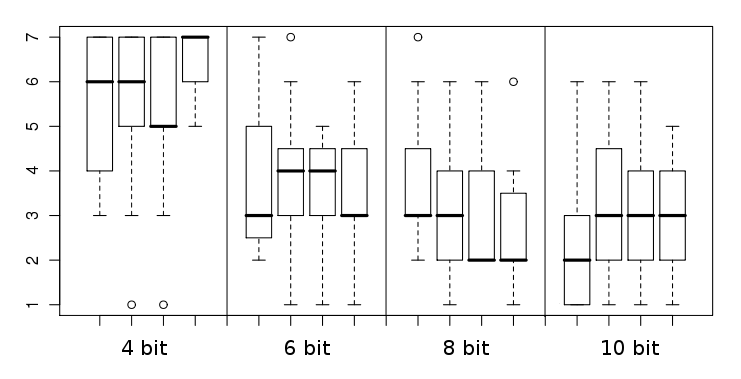
\includegraphics[width=120mm]{boxwhisker_dataset_ballstick}
  \end{center}
  \caption{Box and whisker plot of the different quantisation levels for the
  ball-and-stick visualisation. The results are very similar.}
  \label{fig:results_boxwhisker_dataset_ballstick}
\end{figure}

\begin{figure}
  \begin{center}
    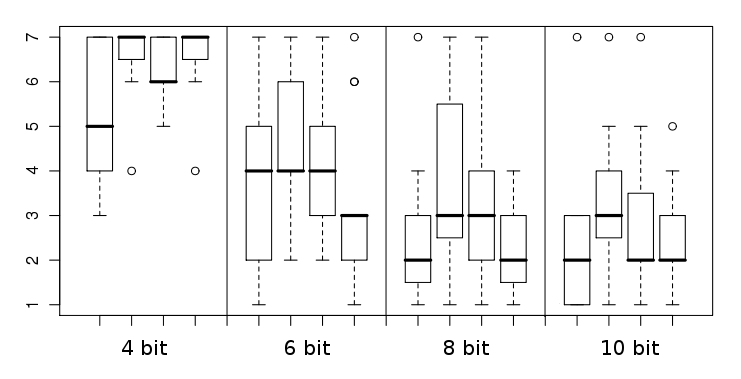
\includegraphics[width=120mm]{boxwhisker_dataset_metaballs}
  \end{center}
  \caption{Box and whisker plot of the different quantisation levels for the
  metaballs visualisation technique. The results are different, but they do
  agree with each other.}
  \label{fig:results_boxwhisker_dataset_metaballs}
\end{figure}

% }}}

\subsection*{Aggregated}
% {{{
\label{sub:results_results_aggregated}

Using the Shapiro-Wilks test for normality on the aggregated data for the ball
and stick, and metaballs visualisation techniques, the null hypothesis of the
Shapiro-Wilks test can be rejected at the 95\% significance level; i.e. the
data is a normal distribution. See Tables
\ref{tab:appendix_ballstick_normality} and
\ref{tab:appendix_metaballs_normality} in Appendix \ref{cha:tables} for the
actual test results.

With the data being verified as a normal distribution, an ANOVA analysis can be
performed. The result from ANOVA analysis indicates that the null hypothesis of
the ANOVA analysis can be rejected at the 99\% significance level, i.e.
quantisation does have a significant perceptual impact. The actual test results
is provided in Tables \ref{tab:appendix_ballstick_anova} and
\ref{tab:appendix_metaballs_anova}.

Tables \ref{tab:appendix_ballstick_tukeyhsd} and
\ref{tab:appendix_metaballs_tukeyhsd} shows the results from performing the
Tukey's HSD analysis on the results from the ball-and-stick, and metaballs
experiments, respectively. The leftmost column shows which of the quantisation
levels are being compared. For ball-and-stick, b4 means quantisation using 4
bits, b6 is 6 bit quantisation, b8 and b10 use 8 and 10 bits, respectively.
Similarly: m4, m6, m8 and m10 means quantisation levels using 4, 6, 8 and 10
bits for the metaballs visualisation technique. The difference between the
means is under the \emph{diff} column, with the lower and upper quartiles in
\emph{lwr} and \emph{upr}, respectively. \emph{p adj} indicates how similar the
factors being compared are.

Inspecting the \emph{p adj} column, 8 and 10 bit quantisation are very similar
(p-value of 0.7135299 and 0.9762546). For between 6 and 8 bit quantisation, the
ball-and-stick visualisation is similar (p-value of 0.2163136) but the values
are significantly different for the metaballs visualisation (p-value of
0.0005950). Using 4 bit quantisation, the values are significantly different
from all the other quantisation levels (p-value of 0.0000000).

Figure \ref{fig:results_boxwhisker_all} is a box and whisker plot showing the
different quantisation levels. The ball-and-stick results are on the left half
of the figure, while the right half is for the metaballs technique. The figure
reflects data from the Tukey's HSD analysis, with 8 and 10 bit quantisation
being similar, 6 and 8 bit less so, and 4 bit quantisation being different from
all the other quantisation levels.

Looking at the box and whisker plot (Figure \ref{fig:results_boxwhisker_all}),
the participants rated 4 bit quantisation as being very different from the
original (median rating of 6 and 7), 6 bit is rated different (median rating of
4), 8 and 10 bit quantisation is rated moderately different (median rating of
3).

\begin{figure}
  \begin{center}
    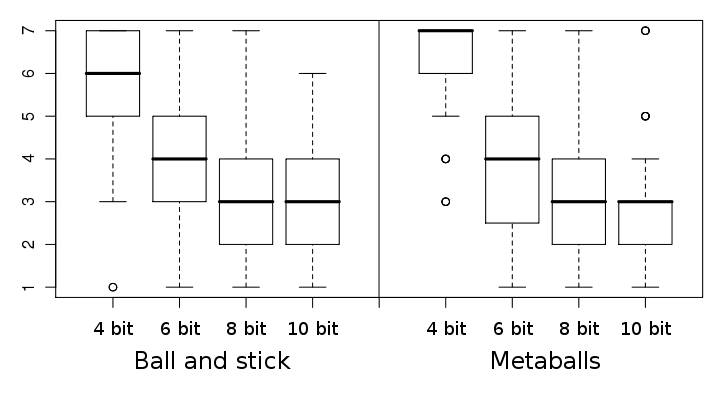
\includegraphics[width=120mm]{boxwhisker_all_both}
  \end{center}
  \caption{Box and whisker plot of the different quantisation levels.}
  \label{fig:results_boxwhisker_all}
\end{figure}

% }}}

% }}}

\section{Discussion}
% {{{
\label{sec:results_discussion}

\subsection*{Dataset specific}
% {{{
\label{sub:results_discussion_dataset}

As mentioned in Section \ref{sub:results_results_dataset}, the Friedman
Test indicates that the different datasets do not have a significant impact on
the results. This means that the perceptually visible effects of quantisation
are similar between datasets.

The effects are not exactly equal due to the size differences in the datasets.
As quantisation produces a limited number of possible values which can be used,
a dataset with larger dimensions will have larger quantisation errors, and thus
more noticeable differences.

However, for datasets with fewer molecules, the bounding box of the data can
shift around as the molecules move. With more molecules, the bounding box is
more likely to remain still as more molecules will need to move in a certain
direction to shift the bounding box. As quantisation allocates values equally
across the bounding box, a shift in the bounding box would cause a
corresponding shift of all the values. In the visualisation, this would be
characterised as the entire volume of data moving around. The simulation would
appear ``wobbly''. The wobbling is more noticeable with quantisation using
fewer bits.

In further analysing the data, there is no consistent increase or decrease in
the noticeable difference with regards to datasets. This may have been as a
result of a number of factors:
\begin{itemize}

  \item participant uncertainty: different participants have their own
  different definitions of ``similar'' and ``different''.

  \item participant bias: participants can be naturally inclined towards
  perceiving similarities, or differences, hence biasing their results.

  \item the quantisation levels were shown in a random order; this may
  influence the participants short-term memory, and thus impact on the
  perceived differences.

  \item large datasets have greater quantisation errors, but the smaller
  datasets ``wobble'', there is thus a visual difference either way.

\end{itemize}

While there are differences as a result of the datasets, the differences are
small and the responses are consistent across datasets.

% }}}

\subsection*{Aggregated}
% {{{
\label{sub:results_discussion_aggregated}

As the dataset does not have a significant impact on the results, all the
results for a specific quantisation level and visualisation technique can be
combined and aggregated together. This allows for a more general analysis of
the effects of quantisation.

The responses from the experiment indicate that 8 and 10 bit quantisation yield
similar results, 6 bit is still similar (but less so), with 4 bit being very
different from the original data. This does reflect the effects of
quantisation. As fewer bits are used, exponentially fewer values are available.
10 bits allows for 1024 possible values, but 4 bits only allows for 16 possible
values. This applies separately to each coordinate. See Table
\ref{tab:results_bitvalues} for an indication of the number of possible values
for each of the quantisation levels.

\begin{table}
  \begin{tabular}{ | l | r | }
  \hline
  Quantisation level & Number of values  \\ \hline
  4 bit              &               16  \\ \hline
  6 bit              &               64  \\ \hline
  8 bit              &              256  \\ \hline
  10 bit             &             1024  \\ \hline
  \end{tabular}
  \caption{Table showing number of values per quantisation level}
  \label{tab:results_bitvalues}
\end{table}

Plotting the means of the quantisation levels (Figure
\ref{fig:results_bm_means}) shows that the metaballs visualisation technique
yields more noticeable differences when using fewer bits, than that of
ball-and-stick.

\begin{figure}
  \begin{center}
    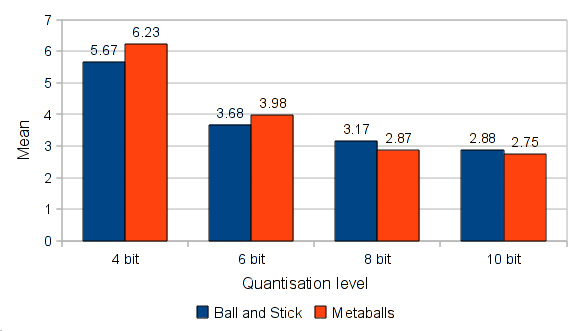
\includegraphics[width=100mm]{bm_means}
  \end{center}
  \caption{Graph showing the mean values of the different quantisation levels}
  \label{fig:results_bm_means}
\end{figure}

As the ball-and-stick visualisation technique shows the individual atoms, it is
easier to see the differences between the original and quantised data. The
spheres are at the actual quantised positions, and quantisation will result in
the spheres being placed in a different position, which is easily noticed.

Due to how the metaballs surface is extracted, the quantisation effects are
very noticeable when using fewer bits. As fewer bits are used, there will be
fewer positions for the water molecules. This distorts the areas of water and
non-water. The resulting extracted surfaces highlights the quantised positions.
See Figure \ref{fig:experiment_metaballs4680}, the quantised water positions
are clearly visible when using 4 bit quantisation.

The quantised water positions are not as clearly visible when using more bits
as the water molecules are placed more accurately, and the water molecules do
not overlap as much.

The metaballs surface is determined by the nearby water molecules, which means
that slight variations in the water molecule positions will not be clearly
reflected in the surface. This explains why the 8 and 10 quantisation levels
are so similar.

% }}}

% }}}

\section{Summary}
% {{{
\label{sec:results_summary}

The statistical analysis shows that the datasets do not have a significant
impact on the results, meaning that the results between datasets are comparably
similar.

Aggregating data from the different datasets together, and analysing this shows
that quantisation levels do have a statistically significant impact on the
perceived difference.

At quantisation levels using fewer bits, the metaballs visualisation technique
is more visually different than that of the ball-and-stick visualisation
technique. Conversely, the ball-and-stick ratings for quantisation levels using
more bits is higher; i.e. the difference from the original data is greater.

Since the perceived difference between 8 and 10 bit quantisation levels is not
statistically significant, 8 bit quantisation is the recommended quantisation
setting. If the data to be compressed is very large, more bits per quantisation
may be needed. However, for data used purely for viewing, 8 bit quantisation is
sufficient.

% }}}

% }}}


\chapter{Conclusion}
% {{{
\label{cha:conclusion}

The visualisation aspect of the water compression system is split into two main
parts. The first part involves visualising the molecular data; both for general
viewing, as well as for supporting the compression aspect of the system. The
second part tests the perceptual impact of quantisation, and allows a decision
on an appropriate level of quantisation to be made.

\section{Visualisation Techniques}
% {{{
\label{sec:conclusion_visualisation}

Five different visualisation techniques have been successfully implemented:
\begin{itemize}

  \item Water Point Visualisation: allows for large areas of water and
  non-water to be see in overview and will be useful for getting an initial
  idea of the volume.

  \item Ball-and-Stick Visualisation: is the traditional approach to
  visualising molecular data, the atoms are represented by spheres and the
  bonds are represented by cylinders.

  \item Metaballs Visualisation: extracts the surface between the water and
  non-water regions of the volume. These regions are clearly separated from
  each other.

  \item Water Cluster Visualisation: shows the extracted water clusters in the
  volume, and is used by the intraframe compression component of the system.

  \item Quantisation Error Visualisation: shows the errors introduced by
  quantisation, which are evenly distributed across the volume.

\end{itemize}

% }}}

\section{Quantisation Experiment}
% {{{
\label{sec:conclustion_experiment}

The results from the quantisation experiment showed that 10 bit and 8 bit
quantisation yield very similar results, and are not rated significantly
different from the original data. Quantisation using 6 bits is still similar,
but the differences are more noticeable. While 4 bit quantisation is rated as
significantly different from the original data, thus, this is thus not
recommended for general use.

The ball-and-stick, and metaballs visualisation techniques perform very
similarly.The ball-and-stick visualisation yields more noticeable differences
when using more bits compared to metaballs, but the metaballs yields more
differences when using fewer bits.

We recommend a maximum quantisation level of 8 bits for visual fidelity. For
large simulations where higher fidelity is needed, then more bits may be used,
but for general viewing, 8 bit quantisation is sufficient.

% }}}

\section{Future work}
% {{{
\label{sec:conclusion_future}

Only two visualisation techniques were tested in the quantisation experiment,
different visualisations may be affected by quantisation differently. Thus,
further experimentation could be conducted to evaluate the effects of
quantisation on other molecular visualisations.

Researchers using the molecular simulations may want to do analysis on the
data, a different quantisation level may be needed due to the different
requirements. Experts in the field would need to be consulted to determine an
acceptable level of quantisation error that can be introduced, this would thus
allow an appropriate quantisation level to be recommended.

The quantisation experiment used participants with no significant background in
chemistry, except for one of the participants. If the participants has more
knowledge of chemistry, they may be able to better notice the effects of
quantisation. An experiment may be conducted using chemists as participants to
determine if their responses are significantly different. The results from this
experiment may change the recommended level of quantisation.

% }}}

% }}}



% \bibliographystyle{abbrvnat}
\bibliographystyle{plain}
\bibliography{report_min}

\appendix
\chapter{Statistical test results}
% {{{
\label{cha:statsresults}

\begin{table}[h!]
  \begin{tabular}{ | l | r | r | }
  \hline
                 & ball and stick p-value & metaballs p-value  \\ \hline
  amall (4 bit)  &                0.02970 &          0.003224  \\ \hline
  cmc (4 bit)    &                0.01617 &         1.056e-05  \\ \hline
  gala (4 bit)   &               0.006227 &          0.002222  \\ \hline
  mscl (4 bit)   &               0.001035 &         1.056e-05  \\ \hline
  \hline

  amall (6 bit)  &              0.06854 * &          0.2670 *  \\ \hline
  gala (6 bit)   &                0.768 * &          0.2008 *  \\ \hline
  cmc (6 bit)    &               0.1263 * &          0.1832 *  \\ \hline
  mscl (6 bit)   &               0.6061 * &          0.008472  \\ \hline
  \hline

  amall (8 bit)  &                0.04416 &          0.003488  \\ \hline
  cmc (8 bit)    &              0.09556 * &         0.05903 *  \\ \hline
  gala (8 bit)   &               0.001952 &          0.1266 *  \\ \hline
  mscl (8 bit)   &                0.02076 &           0.04192  \\ \hline
  \hline

  amall (10 bit) &               0.008083 &         0.0007939  \\ \hline
  cmc (10 bit)   &                0.04372 &          0.3688 *  \\ \hline
  gala (10 bit)  &               0.2525 * &           0.04283  \\ \hline
  mscl (10 bit)  &               0.1550 * &          0.1750 *  \\ \hline
  \end{tabular}
  \caption{shapiro-wilks test results for the different datasets}
  \label{tab:dataset_normality}
\end{table}

a * indicates that the null hypothesis cannot be rejected at the 95\%
confidence interval. i.e. the data is not a normal distribution.


\begin{table}[h!]
  \begin{tabular}{ | l | r | r | r | }
  \hline
                          & chi-squared & df &    p-value  \\ \hline
  Ball and stick (4 bit)  &      3.9921 &  3 &     0.2623  \\ \hline
  Ball and stick (6 bit)  &      0.4545 &  3 &     0.9288  \\ \hline
  Ball and stick (8 bit)  &         6.6 &  3 &     0.0858  \\ \hline
  Ball and stick (10 bit) &     25.8416 &  3 &  1.029e-05  \\ \hline
  Metaballs (4 bit)       &      4.4851 &  3 &     0.2136  \\ \hline
  Metaballs (6 bit)       &      7.1957 &  3 &    0.06592  \\ \hline
  Metaballs (8 bit)       &      3.9778 &  3 &     0.2639  \\ \hline
  Metaballs (10 bit)      &      5.0294 &  3 &     0.1697  \\ \hline
  \end{tabular}
  \caption{Friedman Test results for the different quantisation levels}
  \label{tab:friedman_test_results}
\end{table}


\begin{table}[h!]
  \begin{tabular}{ | l | r | r | }
  \hline
  Quantistion level &      W &   p-value  \\ \hline
  4 bit             & 0.8235 & 5.487e-07  \\ \hline
  6 bit             & 0.9488 &   0.01366  \\ \hline
  8 bit             & 0.8865 & 4.405e-05  \\ \hline
  10 bit            & 0.8999 & 0.0001304  \\ \hline
  \end{tabular}
  \caption{Shapiro-Wilks test results for the ball and stick visualisation
  technique}
  \label{tab:ballstick_normality}
\end{table}


\begin{table}[h!]
  \begin{tabular}{ | l | r | r | r | r | r | }
  \hline
               &  Df & Sum Sq & Mean Sq & F value &   Pr($>$F)   \\ \hline
  quantisation &   3 & 283.77 &   94.59 &  44.218 & $<$ 2.2e-16  \\ \hline
  Residuals    & 236 & 504.83 &    2.14 &         &              \\ \hline
  \end{tabular}
  \caption{ANOVA analysis of the ball and stick visualisation technique}
  \label{tab:ballstick_anova}
\end{table}


\begin{table}[h!]
  \begin{tabular}{ | l | r | r | }
  \hline
  Quantistion level &      W &   p-value  \\ \hline
  4 bit             & 0.6942 & 6.857e-10  \\ \hline
  6 bit             & 0.9244 &  0.001164  \\ \hline
  8 bit             & 0.8788 & 2.407e-05  \\ \hline
  10 bit            & 0.8722 & 1.466e-05  \\ \hline
  \end{tabular}
  \caption{Shapiro-Wilks test results for the metaballs visualisation
  technique}
  \label{tab:metaballs_normality}
\end{table}


\begin{table}[h!]
  \begin{tabular}{ | l | r | r | r | r | r | }
  \hline
               &  Df & Sum Sq & Mean Sq & F value &    Pr($>$F)  \\ \hline
  quantisation &   3 & 469.68 &  156.56 &  65.291 & $<$ 2.2e-16  \\ \hline
  Residuals    & 236 & 565.90 &    2.40 &         &              \\ \hline
  \end{tabular}
  \caption{ANOVA analysis of the metaballs visualisation technique}
  \label{tab:metaballs_anova}
\end{table}



\begin{table}[h!]
  \begin{tabular}{ | l | r | r | r | }
  \hline
                          &  Mean & Median & Mode  \\ \hline
  Ball and stick (4 bit)  & 5.667 &      6 &    7  \\ \hline
  Ball and stick (6 bit)  & 3.683 &      4 &    3  \\ \hline
  Ball and stick (8 bit)  & 3.167 &      3 &    2  \\ \hline
  Ball and stick (10 bit) & 2.883 &      3 &    2  \\ \hline
  Metaballs (4 bit)       & 6.233 &      7 &    7  \\ \hline
  Metaballs (6 bit)       & 3.983 &      4 &    2  \\ \hline
  Metaballs (8 bit)       & 2.867 &      3 &    2  \\ \hline
  Metaballs (10 bit)      &  2.75 &      3 &    3  \\ \hline
  \end{tabular}
  \caption{Statistics for the two visualisation techniques and different
  quantisation levels}
  \label{tab:experiment_statistics}
\end{table}


% }}}



\end{document}
